\documentclass[12pt, twoside]{article}
\usepackage[letterpaper, margin=1in, headsep=0.5in]{geometry}
\usepackage[english]{babel}
\usepackage[utf8]{inputenc}
\usepackage{amsmath}
\usepackage{amsfonts}
\usepackage{amssymb}
\usepackage{tikz}
\usetikzlibrary{quotes, angles}
\usepackage{graphicx}
\usepackage{enumitem}
\usepackage{multicol}

\newif\ifmeta
\metatrue %print standards and topics tags

\title{Regents Geometry}
\author{Chris Huson}
\date{September 2020}

\usepackage{fancyhdr}
\pagestyle{fancy}
\fancyhf{}
\renewcommand{\headrulewidth}{0pt} % disable the underline of the header
\raggedbottom


\fancyhead[LE]{\thepage}
\fancyhead[RO]{\thepage \\ Name: \hspace{4cm} \,\\}
\fancyhead[LO]{BECA / Dr. Huson / Geometry 02 Area and volume}

\begin{document}

\subsubsection*{2.3 CW Compound areas}
\begin{enumerate}
\item Do Now: The ray $\overrightarrow{KM}$ bisects $\angle JKL$. Given $m\angle JKM = 4x-20$ and \\$m\angle MKL = 3x+4$. Identify the true statement(s).
 \begin{multicols}{2}
    \begin{enumerate}
      \item $\angle JKM$ and $\angle MKL$ are a linear pair\\
      $(4x-20) + (3x+4)=180^\circ$
      \item $\angle JKM$, $\angle MKL$ are adjacent and\\
      $4x-20 =90^\circ$
      \item $\angle JKM \cong \angle MKL$\\
      $4x-20 = 3x+4$
  \end{enumerate}
  \begin{center}
    \begin{tikzpicture}[scale=0.6, rotate=-10]
      \draw [<->, thick] (160:5)node[below left]{$J$} 
      --(0,0)node[below left]{$K$}
      --(10:5)node[above right]{$L$};
      \draw [->, thick] (0,0)--(90:5)node[below left]{$M$};
      %\draw [fill] (0,0) circle [radius=0.05] node[below]{$A$};
      %\draw [fill] (5,0) circle [radius=0.05] node[below]{$B$};
    \end{tikzpicture}
  \end{center}
\end{multicols}
Copy the correct equation and find $m\angle JKL$. Check your answer. \vspace{8cm}

\item Find the area of the shape shown below. All angles are $90^\circ$.\hfill \emph{(not drawn to scale)}
    \begin{flushleft}
    \begin{tikzpicture}
      \draw [-, thick] (0,0)--(5,0)--(5,2)--(3,2)--(3,6)--(0,6)--cycle;
      %\draw [fill] (0,0) circle [radius=0.05] node[left]{$A$};
      %\draw [fill] (7,0) circle [radius=0.05] node[right]{$B$};
      %\draw [fill] (7,2) circle [radius=0.05] node[right]{$C$};
      %\draw [fill] (0,2) circle [radius=0.05] node[left]{$D$};
      \node at (5.5, 1){4};
      \node at (4, 2.5){4};
      \node at (2.5, -0.5){10};
      \node at (-0.5, 3){12};
    \end{tikzpicture}
    \end{flushleft}

\newpage
\item Find the area of $\triangle ABC$. The altitude $h$ of the triangle is $4 \frac{3}{4}$ centimeters and the base $AB=9 \frac{1}{2}$ cm. (diagram not to scale) \\[0.5cm]
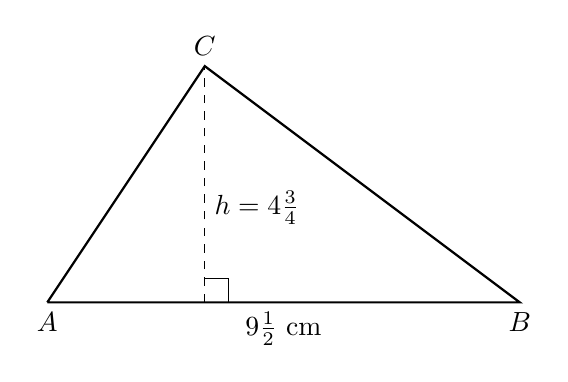
\begin{tikzpicture}[scale=1.]
  \draw [thick]
    (2,0)node[below]{$A$}--
    (8,0)node[below]{$B$}--
    (4,3)node[above]{$C$} --(2,0);
 \draw [dashed] (4,0)--(4,3);
 \draw (4,0)++(0.3,0)--++(0,0.3)--+(-0.3,0);
 \node at (4,1.2)[right]{$h=4 \frac{3}{4}$};
 \node at (5,0)[below]{$9 \frac{1}{2}$ cm};
\end{tikzpicture} 

\item Find the area $A$ of the shape shown below in terms of unit squares.
    \begin{flushleft}
      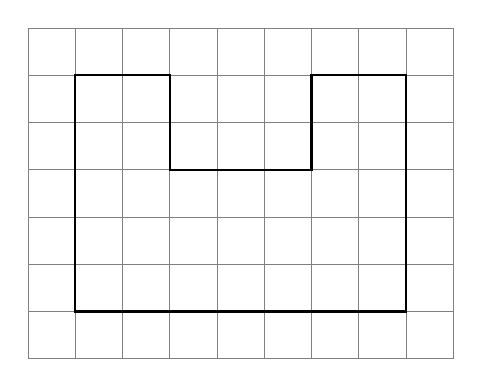
\begin{tikzpicture}[scale=0.6]
        \draw [help lines] (-4,-4) grid (5,3);
        \draw [thick, -] (-3,-3)--(4,-3)--(4,2)--(2,2)--(2,0)--(-1,0)--(-1,2)--(-3,2)--cycle;
      \end{tikzpicture}
    \end{flushleft}

\item Find the area of shape $ABCDE$ below, a triangle on a rectangle. The altitude $h$ of the triangle is $3.20$ centimeters and the base $AB=5.5$ cm. The rectangle is 1 cm tall. (diagram not to scale) \\[0.5cm]
      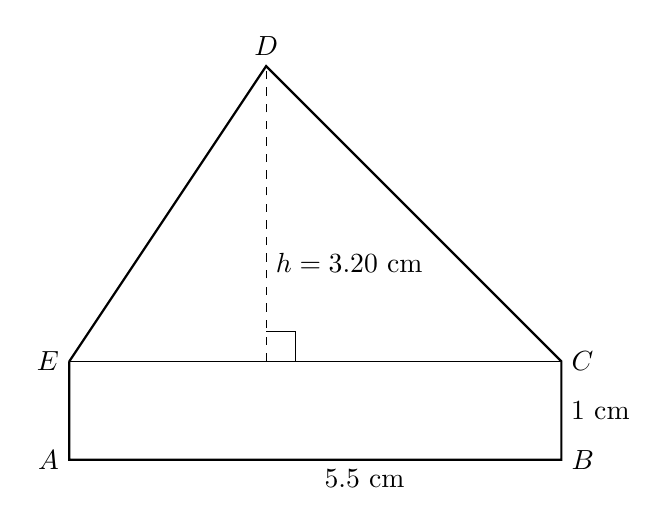
\begin{tikzpicture}[scale=1.25]
        \draw (2,0)--(7,0);
        \draw [thick] 
          (2,0)node[left]{$E$}--
          (2,-1)node[left]{$A$}--
          (7,-1)node[right]{$B$}--
          (7,0)node[right]{$C$}--
          (4,3)node[above]{$D$}--(2,0);
        \draw [dashed] (4,0)--(4,3);
        \draw (4,0)++(0.3,0)--++(0,0.3)--+(-0.3,0);
        \node at (4,1)[right]{$h=3.20$ cm};
        \node at (5,-1)[below]{$5.5$ cm};
        \node at (7,-0.5)[right]{$1$ cm};
      \end{tikzpicture} \vspace{1.0cm}


\end{enumerate}
\end{document}